\documentclass[
    11pt, % Set the default font size, options include: 8pt, 9pt, 10pt, 11pt, 12pt, 14pt, 17pt, 20pt
    %
    aspectratio=169, % Uncomment to set the aspect ratio to a 16:9 ratio which matches the aspect ratio of 1080p and 4K screens and projectors
]{beamer}

\graphicspath{{Images/}{./}} % Specifies where to look for included images (trailing slash required)
\usepackage{booktabs} % Allows the use of \toprule, \midrule and \bottomrule for better rules in tables

%\usepackage{appendixnumberbeamer} %If you want a separate slide counter for your appendix

%%% Customize Theme %%%%%%%%%%%%%%%%%%%%%%
\usetheme{Madrid} % You can use other themes too, but this changes many things. I've found Madrid to be the best for this color scheme

%fg = font color
%bg = background color

% ! WARNING ! : Many colors are linked to multiple attributes, so changing one color can have unexpected changes!

% If you want to tweak the shading of colors, tweak the below 2 lines:
\definecolor{myBlue}{RGB}{20, 20, 255}
\definecolor{myTeal}{RGB}{102, 51, 153}

% Bottom right hand color
\setbeamercolor*{structure}{bg=myBlue!20,fg=myBlue!90}

\setbeamercolor*{palette primary}{use=structure,fg=white,bg=structure.fg} %?
\setbeamercolor*{palette secondary}{use=structure,fg=myBlue,bg=white}
    %bottom left of footer & bar between title & top bubbles
\setbeamercolor*{palette tertiary}{use=structure,fg=white,bg=myBlue}

\setbeamercolor{frametitle}{bg=myBlue!85,fg=white} %title of each slide

\setbeamercolor*{titlelike}{parent=palette primary} %?
%\setbeamercolor{titlelike}{parent=palette primary,fg=structure.fg!50!myBlue}

%for miniframe (very top) AND center footer
\setbeamercolor{section in head/foot}{fg=myTeal, bg=white}

%%% Specific Colors %%%
\setbeamercolor{item projected}{bg=myTeal}
\setbeamertemplate{enumerate items}{bg=myTeal}

\setbeamercolor{itemize item}{fg=myTeal}
\setbeamercolor{itemize subitem}{fg=myTeal}

\setbeamercolor{button}{bg=myTeal}

%%% Edits ONLY the TOC slide %%%
\setbeamercolor{section in toc}{fg=black}
\setbeamercolor{subsection in toc}{fg=black}

%%% Block Colors %%%
% Standard block %
    \setbeamercolor{block title}{bg=myTeal, fg=white}
    \setbeamercolor{block body}{bg=myTeal!20}

% Alerted block % If you want to customize it's color
    %\setbeamercolor{block title alerted}{bg=cyan, fg=white}
    %\setbeamercolor{block body alerted}{bg=cyan!10}

% Example block % If you want to customize it's color
    %\setbeamercolor{block title example}{bg=cyan, fg=white}
    %\setbeamercolor{block body example}{bg=cyan!10}

%---------------------------------------------------------
%	SELECT FONT THEME & FONTS
%---------------------------------------------------------
\usefonttheme{default} % Typeset using the default sans serif font
\usepackage{palatino} % Use the Palatino font for serif text
\usepackage[default]{opensans} % Use the Open Sans font for sans serif text
\useinnertheme{circles}

%---------------------------------------------------------
%	SELECT OUTER THEME
%---------------------------------------------------------
% Outer themes change the overall layout of slides, such as: header and footer lines, sidebars and slide titles. Uncomment each theme in turn to see what changes it makes to your presentation.

%\useoutertheme{default}
%
\useoutertheme{miniframes}

%\useoutertheme{infolines}
%\useoutertheme{smoothbars}
%\useoutertheme{sidebar}
%\useoutertheme{split}
%\useoutertheme{shadow}
%\useoutertheme{tree}
%\useoutertheme{smoothtree}

%---------------------------------------------------------
%	PRESENTATION INFORMATION
%---------------------------------------------------------

\title[Multi-Agent RL for Spacecraft Guidance]{Robust Reinforcement Learning Differential Game Guidance in Low-Thrust, Multi-Body Dynamical Environments}
\subtitle{A Zero-Sum Reinforcement Learning Approach in Three-Body Dynamics}
\author[Ali Baniasad]{Ali Baniasad \\ \smallskip Supervisor: Dr. Nobahari}

\institute[]{Department of Aerospace Engineering \\ \smallskip Sharif University of Technology}
\date[\today]

\logo{
\includegraphics[width=1.cm]{sharif_logo.png}}

%---------------------------------------------------------
%---------------------------------------------------------
%---------------------------------------------------------
\begin{document}

%---------------------------------------------------------
%	TITLE SLIDE
%---------------------------------------------------------
\section{}
\begin{frame}
	\titlepage % Output the title slide, automatically created using the text entered in the PRESENTATION INFORMATION block above

\end{frame}

%---------------------------------------------------------
%	TABLE OF CONTENTS SLIDE
%---------------------------------------------------------

\begin{frame}
	\frametitle{Outline}

	\tableofcontents
\end{frame}

%---------------------------------------------------------
%	PRESENTATION BODY SLIDES
%---------------------------------------------------------

\section{Introduction \& Motivation}

%------------------------------------------------
\begin{frame}
	\frametitle{Research Motivation}
	
	\begin{itemize}
		\item \textbf{Space missions} increasingly require autonomous guidance systems
		\item \textbf{Low-thrust spacecraft} operate in complex gravitational environments
		\item \textbf{Three-body dynamics} (Earth-Moon CRTBP) present inherent instabilities
		\item \textbf{Classical control methods} struggle with:
		\begin{itemize}
			\item Model uncertainties
			\item Environmental disturbances
			\item Fuel efficiency requirements
		\end{itemize}
		\item \textbf{Need for robust, adaptive guidance} without precise dynamic models
	\end{itemize}
	
	\vspace{0.3cm}
	\begin{center}
		\textit{How can we achieve robust spacecraft guidance in uncertain environments?}
	\end{center}
\end{frame}

%------------------------------------------------
\begin{frame}
	\frametitle{Problem Statement}
    \vspace{-0.35cm}
	\begin{block}{Research Objective}
		Design a robust guidance framework for low-thrust spacecraft operating in Earth-Moon three-body dynamics under uncertainties.
	\end{block}
	
	\begin{columns}[t]
		\begin{column}{0.5\textwidth}
			\textbf{System Characteristics:}
			\begin{itemize}
				\item State: $\mathbf{x} = [x, y, \dot{x}, \dot{y}]^T$
				\item Control: $\mathbf{u} \leq u_{\max}$
				\item Dynamics: $\dot{\mathbf{x}} = f(\mathbf{x}, \mathbf{u})$
			\end{itemize}
		\end{column}
		\begin{column}{0.5\textwidth}
			\textbf{Mission Environment:}
			\begin{itemize}
				\item Earth-Moon CRTBP
				\item Lyapunov orbit transfer
				\item Low-thrust propulsion
				% \item Real-time constraints
			\end{itemize}
		\end{column}
	\end{columns}
	
	% \vspace{-0.}
    \begin{minipage}
        {0.93\textwidth}
            \begin{exampleblock}{Mathematical Formulation}
		Optimal control problem with state-dependent uncertainties and adversarial disturbances
	\end{exampleblock}
    \end{minipage}
\end{frame}

%------------------------------------------------
\begin{frame}
    \frametitle{Problem Statement - Challenges \& Approach}
    
    \begin{columns}[T,onlytextwidth]
        \begin{column}{0.45\textwidth}
            \textbf{Uncertainty Sources:}
            \begin{itemize}
                \item Random initial conditions
                \item Actuator disturbances
                \item Sensor noise
                \item Model mismatch
                \item Communication delays
                \item External perturbations
            \end{itemize}
        \end{column}
        \begin{column}{0.55\textwidth}
            \textbf{Design Requirements:}
            \begin{itemize}
                \item Robust performance
                \item Fuel efficiency
                \item Real-time capability
                \item Model-free approach
                \item Adaptive behavior
                \item Safety guarantees
            \end{itemize}
        \end{column}
    \end{columns}
    
    \vspace{-0.1cm}
    \begin{minipage}
        {0.93\textwidth}
            \begin{alertblock}{Key Challenge}
        Formulate as zero-sum differential game: spacecraft vs. environmental disturbances
    \end{alertblock}
    \end{minipage} 

\end{frame}

    
%------------------------------------------------
\section{Methodology}

%------------------------------------------------
\begin{frame}
	\frametitle{Multi-Agent Reinforcement Learning Framework}
	
	\begin{columns}[t]
		\begin{column}{0.6\textwidth}
			\textbf{Game-Theoretic Formulation:}
			\begin{itemize}
				\item \textbf{Player 1}: Controller agent (spacecraft)
				\item \textbf{Player 2}: Adversary agent (disturbances)
				\item \textbf{Objective}: Zero-sum differential game
			\end{itemize}
			
			\vspace{0.3cm}
			\textbf{Training Paradigm:}
			\begin{itemize}
				\item Centralized training
				\item Decentralized execution
				% \item Shared actor-critic networks
			\end{itemize}
		\end{column}
		\begin{column}{0.4\textwidth}
			\begin{figure}
				\centering
				
\includegraphics[width=\textwidth]{framework_diagram.png}
				\caption{MARL Framework}
			\end{figure}
		\end{column}
	\end{columns}
	
	\begin{exampleblock}{Innovation}
		Extension of single-agent RL algorithms (DDPG, TD3, SAC, PPO) to multi-agent zero-sum variants (MA-DDPG, MATD3, MASAC, MAPPO)
	\end{exampleblock}
\end{frame}

%------------------------------------------------
\begin{frame}
	\frametitle{Algorithm Extensions}
	
	\begin{block}{Single-Agent $\rightarrow$ Multi-Agent Zero-Sum}
		Extended four continuous RL algorithms to handle adversarial scenarios
	\end{block}
	
	\begin{columns}[t]
		\begin{column}{0.5\textwidth}
			\textbf{DDPG $\rightarrow$ MA-DDPG}
			\begin{itemize}
				\item Deterministic policy gradient
				\item Experience replay
				\item Target networks
			\end{itemize}
			
			% \vspace{0.1cm}
			\textbf{SAC $\rightarrow$ MA-SAC}
			\begin{itemize}
				\item Entropy regularization
				\item Stochastic policies
				\item Automatic temperature tuning
			\end{itemize}
		\end{column}
		\begin{column}{0.5\textwidth}
			\textbf{TD3 $\rightarrow$ MA-TD3}
			\begin{itemize}
				\item Twin critic networks
				\item Delayed policy updates
				\item Target policy smoothing
			\end{itemize}
			
			% \vspace{0.1cm}
			\textbf{PPO $\rightarrow$ MA-PPO}
			\begin{itemize}
				\item Proximal policy optimization
				\item Clipped surrogate objective
				\item On-policy learning
			\end{itemize}
		\end{column}
	\end{columns}
\end{frame}

%------------------------------------------------
\begin{frame}
	\frametitle{Network Architecture}
	
	\begin{columns}[t]
		\begin{column}{0.5\textwidth}
			\textbf{Actor-Critic Structure:}
			\begin{itemize}
				\item 3 hidden layers
				\item 32 neurons per layer
				\item ReLU activation
				\item Learning rate: $3 \times 10^{-4}$
			\end{itemize}
			
			\vspace{0.3cm}
			\textbf{Training Parameters:}
			\begin{itemize}
				\item 1M environment steps
				\item Batch size: 1024
				\item Buffer size: 100K
				\item Adam optimizer
			\end{itemize}
		\end{column}
		\begin{column}{0.5\textwidth}
			\begin{figure}
				\centering
				
\includegraphics[width=\textwidth]{network_architecture.png}
				\caption{Network Structure}
			\end{figure}
		\end{column}
	\end{columns}
	
	\begin{block}{Shared Networks}
		Both agents use identical network architectures with separate parameter sets for competitive learning
	\end{block}
\end{frame}

%------------------------------------------------
\section{Experimental Setup}

%------------------------------------------------
\begin{frame}
	\frametitle{Evaluation Scenarios}
	
	\begin{block}{Mission: Transfer to Earth-Moon Lyapunov Orbit}
		Circular Restricted Three-Body Problem (CRTBP) environment
	\end{block}
	
	\begin{columns}[t]
		\begin{column}{0.5\textwidth}
			\textbf{Uncertainty Scenarios:}
			\begin{enumerate}
				\item Random initial states ($\sigma = 0.1$)
				\item Actuator disturbances ($\sigma = 0.05$)
				\item Model mismatch ($\sigma = 0.05$)
				\item Partial observations (50\% missing)
				\item Sensor noise ($\sigma = 0.05$)
				\item Communication delays (10 steps)
			\end{enumerate}
		\end{column}
		\begin{column}{0.5\textwidth}
			\textbf{Performance Metrics:}
			\begin{itemize}
				\item Trajectory accuracy
				\item Fuel consumption
				\item System stability
				\item Convergence rate
				\item Robustness measures
			\end{itemize}
			
			% \vspace{0.3cm}
			\textbf{Baseline Comparison:}
			\begin{itemize}
				\item Single-agent variants
				% \item Classical LQR/LQG
				% \item Model predictive control
			\end{itemize}
		\end{column}
	\end{columns}
\end{frame}

%------------------------------------------------
\section{Results}

%------------------------------------------------
\begin{frame}
	\frametitle{Trajectory Comparison: MA-TD3 Performance}
	\vspace{-.75cm}
	\begin{columns}[t]
		\begin{column}{0.5\textwidth}
			\begin{figure}
				\centering
				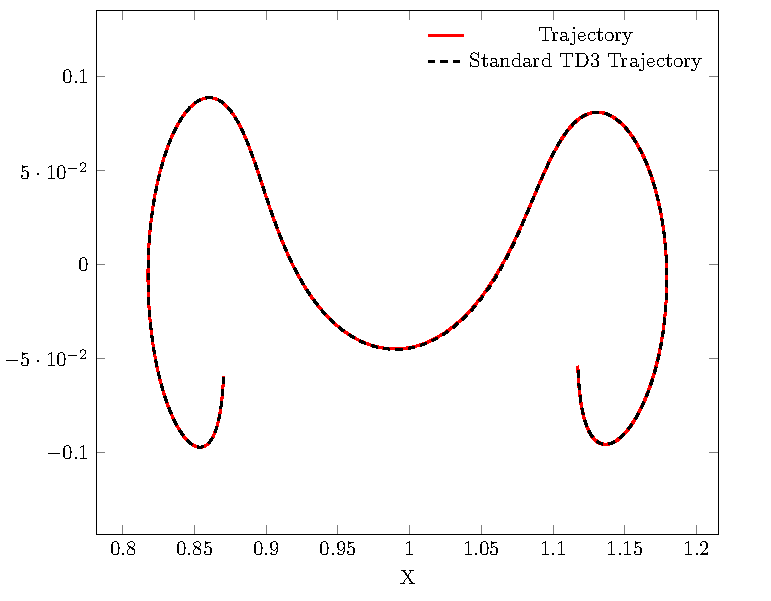
\includegraphics[width=.7\textwidth]{../../Report/plots/td3/trajectory_force/plot_trajectory}
				\vspace{-.5cm}
				\caption{Single-Agent vs Multi-Agent TD3}
			\end{figure}
		\end{column}
		\begin{column}{0.5\textwidth}
			\begin{figure}
				\centering
				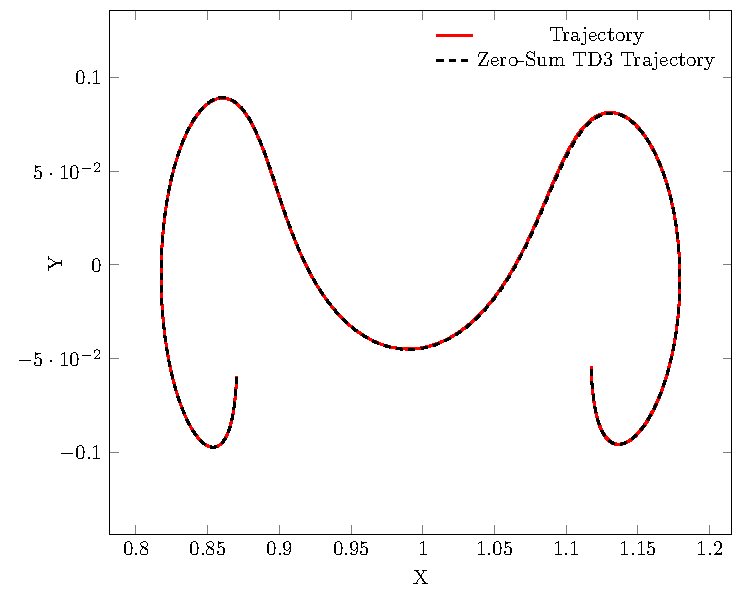
\includegraphics[width=.7\textwidth]{../../Report/plots/td3/trajectory_force/plot_trajectory_zs}
				\vspace{-.5cm}
				\caption{Thrust Commands}
			\end{figure}
		\end{column}
	\end{columns}
	\vspace{-0.5cm}
	\begin{alertblock}{Key Observation}
		Zero-sum variants demonstrate more direct trajectories with smoother thrust profiles and reduced fuel consumption
	\end{alertblock}
\end{frame}

%------------------------------------------------
\begin{frame}
	\frametitle{Robustness Evaluation Results}
	
	\begin{figure}
		\centering
		
\includegraphics[width=0.9\textwidth]{robustness_comparison_all.png}
		\caption{Performance under different uncertainty scenarios}
	\end{figure}
	
	\begin{block}{Key Findings}
		\begin{itemize}
			\item Zero-sum variants consistently outperform single-agent baselines
			\item MATD3 shows best overall performance across all scenarios
			\item Significant improvements in sensor noise and time delay scenarios
		\end{itemize}
	\end{block}
\end{frame}

%------------------------------------------------
\begin{frame}
	\frametitle{Algorithm Performance Comparison}
	
	\begin{columns}[t]
		\begin{column}{0.5\textwidth}
			\textbf{Single-Agent Algorithms:}
			\begin{figure}
				\centering
				
\includegraphics[width=\textwidth]{single_agent_comparison.png}
				\caption{Standard RL Performance}
			\end{figure}
		\end{column}
		\begin{column}{0.5\textwidth}
			\textbf{Multi-Agent Zero-Sum:}
			\begin{figure}
				\centering
				
\includegraphics[width=\textwidth]{multi_agent_comparison.png}
				\caption{Zero-Sum RL Performance}
			\end{figure}
		\end{column}
	\end{columns}
	
	\begin{exampleblock}{Best Performer}
		MATD3 achieves optimal trade-off between trajectory accuracy and propellant consumption while maintaining stability in harsh conditions
	\end{exampleblock}
\end{frame}

%------------------------------------------------
\section{Hardware Implementation}

%------------------------------------------------
\begin{frame}
	\frametitle{Real-Time Deployment}
	
	\begin{columns}[t]
		\begin{column}{0.5\textwidth}
			\textbf{Optimization Techniques:}
			\begin{itemize}
				\item INT8 quantization
				\item ONNX format export
				\item ROS 2 integration
				\item Hardware-in-the-loop testing
			\end{itemize}
			
			\vspace{0.3cm}
			\textbf{Performance Metrics:}
			\begin{itemize}
				\item Inference time: 5.8 ms
				\item Memory usage: 9.2 MB
				\item Control frequency: 100 Hz
				\item Zero deadline misses
			\end{itemize}
		\end{column}
		\begin{column}{0.5\textwidth}
			\begin{figure}
				\centering
				
\includegraphics[width=\textwidth]{deployment_architecture.png}
				\caption{ROS 2 Deployment Architecture}
			\end{figure}
		\end{column}
	\end{columns}
	
	\begin{block}{Optimization Results}
		47\% improvement in latency and 53\% reduction in memory footprint compared to FP32 models
	\end{block}
\end{frame}

%------------------------------------------------
\section{Contributions \& Conclusions}

%------------------------------------------------
\begin{frame}
	\frametitle{Research Contributions}
	
	\begin{enumerate}
		\item \textbf{Novel Framework Development}
		\begin{itemize}
			\item First multi-agent zero-sum RL framework for spacecraft guidance in CRTBP
			\item Game-theoretic formulation for robust control under uncertainties
		\end{itemize}
		
		\item \textbf{Algorithm Extensions}
		\begin{itemize}
			\item Extended four major RL algorithms to multi-agent zero-sum variants
			\item Comprehensive performance analysis across uncertainty scenarios
		\end{itemize}
		
		\item \textbf{Practical Implementation}
		\begin{itemize}
			\item Real-time deployment with quantization and optimization
			\item Hardware-in-the-loop validation on ROS 2 platform
		\end{itemize}
		
		\item \textbf{Performance Validation}
		\begin{itemize}
			\item Demonstrated superior robustness compared to classical methods
			\item Quantified improvements in fuel efficiency and trajectory accuracy
		\end{itemize}
	\end{enumerate}
\end{frame}

%------------------------------------------------
\begin{frame}
	\frametitle{Conclusions}
	
	\begin{block}{Main Findings}
		\begin{itemize}
			\item Multi-agent zero-sum RL enables robust spacecraft guidance without precise dynamic models
			\item MATD3 delivers optimal performance across all evaluation scenarios
			\item Framework is ready for practical deployment with real-time constraints
		\end{itemize}
	\end{block}
	
	\begin{columns}[t]
		\begin{column}{0.5\textwidth}
			\textbf{Advantages:}
			\begin{itemize}
				\item Model-free approach
				\item Adaptive to uncertainties
				\item Fuel-efficient trajectories
				\item Real-time capability
			\end{itemize}
		\end{column}
		\begin{column}{0.5\textwidth}
			\textbf{Future Work:}
			\begin{itemize}
				\item 3D CRTBP extension
				\item Multi-body dynamics
				\item Swarm coordination
				\item Deep space missions
			\end{itemize}
		\end{column}
	\end{columns}
	
	\vspace{0.3cm}
	\begin{center}
		\textbf{The framework opens new possibilities for autonomous space exploration}
	\end{center}
\end{frame}

%---------------------------------------------------------
%	CLOSING SLIDE
%---------------------------------------------------------

% To remove miniframe from top
\appendix
\setbeamertemplate{headline}{}
\addtobeamertemplate{frametitle}{\vspace*{-\headheight}}{}

\begin{frame}[noframenumbering]
	\begin{center}
		{\LARGE Thank You!}
		
		\vspace{1cm}
		
		{\large Questions \& Discussion}
		
		\vspace{1cm}
		
			\textit{Ali Baniasad} 
			% extit{alibaniasad1999@gmail.com} 
		
		\vspace{0.5cm}
		
		Department of Aerospace Engineering \\ 
		Sharif University of Technology
	\end{center}
\end{frame}

%---------------------------------------------------------
%	APPENDIX SLIDES
%---------------------------------------------------------

%------------------------------------------------
\begin{frame}[noframenumbering]
\label{Technical Details}
	\frametitle{Appendix - Technical Implementation Details}
	
	\begin{columns}[t]
		\begin{column}{0.5	extwidth}
				extbf{Environment Setup:}
			\begin{itemize}
				\item PyTorch \& OpenAI Gym
				\item CRTBP dynamics implementation
				\item Custom reward function design
				\item Parallel environment execution
			\end{itemize}
			
			\vspace{0.3cm}
			
				extbf{Network Architecture:}
			\begin{itemize}
				\item Input: 4D state vector
				\item Hidden: 3 layers × 256 neurons
				\item Output: 2D action vector (thrust)
				\item Activation: ReLU
			\end{itemize}
		\end{column}
		\begin{column}{0.5	extwidth}
				extbf{Training Configuration:}
			\begin{itemize}
				\item Episodes: 1M steps
				\item Batch size: 1024
				\item Learning rate: 3e-4
				\item Discount factor: 0.99
				\item Replay buffer: 100K
			\end{itemize}
			
			\vspace{0.3cm}
			
				extbf{Evaluation Metrics:}
			\begin{itemize}
				\item Cumulative reward
				\item Trajectory deviation
				\item Fuel consumption
				\item Convergence stability
			\end{itemize}
		\end{column}
	\end{columns}
\end{frame}

%------------------------------------------------
\begin{frame}[noframenumbering]
\label{Algorithm Details}
	\frametitle{Appendix - Zero-Sum Algorithm Extensions}
	
	\begin{block}{MATD3 Algorithm Highlights}
		\begin{itemize}
			\item Twin critic networks to reduce overestimation bias
			\item Delayed policy updates for stability
			\item Target policy smoothing for robustness
			\item Competitive training between agents
		\end{itemize}
	\end{block}
	
	\begin{columns}[t]
		\begin{column}{0.5	extwidth}
				extbf{Key Modifications:}
			\begin{enumerate}
				\item Shared environment state
				\item Adversarial action selection
				\item Minimax objective function
				\item Nash equilibrium convergence
			\end{enumerate}
		\end{column}
		\begin{column}{0.5	extwidth}
				extbf{Performance Benefits:}
			\begin{enumerate}
				\item Enhanced robustness
				\item Better generalization
				\item Improved worst-case handling
				\item Stable learning dynamics
			\end{enumerate}
		\end{column}
	\end{columns}
\end{frame}

%------------------------------------------------
\begin{frame}[noframenumbering]
\label{Future Work}
	\frametitle{Appendix - Future Research Directions}
	
	\begin{enumerate}
		\item 	extbf{Multi-Body Extensions}
		\begin{itemize}
			\item Sun-Earth-Moon system
			\item Jupiter-Europa dynamics
			\item Asteroid belt navigation
		\end{itemize}
		
		\item 	extbf{Swarm Coordination}
		\begin{itemize}
			\item Formation flying control
			\item Distributed decision making
			\item Communication constraints
		\end{itemize}
		
		\item 	extbf{Advanced Techniques}
		\begin{itemize}
			\item Meta-learning approaches
			\item Hierarchical reinforcement learning
			\item Physics-informed neural networks
		\end{itemize}
		
		\item 	extbf{Mission Applications}
		\begin{itemize}
			\item Lunar gateway operations
			\item Deep space exploration
			\item Interplanetary transfers
		\end{itemize}
	\end{enumerate}
\end{frame}

%------------------------------------------------
\begin{frame}[noframenumbering]
\label{Figure}
	\frametitle{Appendix - A figure}
        \hyperlink{Test}{\beamerreturnbutton{Return to presentation}}

        \begin{figure}[h!]
            \centering
            %\caption{}
            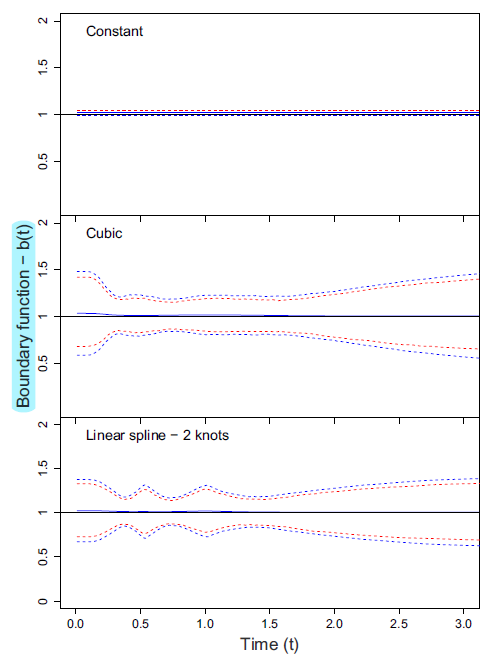
\includegraphics[angle=0, width=5cm]{Newey et al Graph.png}
            %\label{fig}
        \end{figure}
\end{frame}

%------------------------------------------------
\begin{frame}[noframenumbering]
\label{Terms}
	\frametitle{Appendix - Terms}

        \begin{columns}[t] % The "c" option specifies centered vertical alignment while the "t" option is used for top vertical alignment
		\begin{column}{0.5\textwidth} % Right column width
                Some Estimators:
                \begin{itemize}
                    \item Drift: $\hat{\delta}$
                    \item Boundary: $\hat{b}(t)$
                \end{itemize}
		\end{column}
  		\begin{column}{0.5\textwidth} % Left column width
                Some Variables:
                \begin{itemize}
                    \item $\hat{V}$
                    \item $\hat{m}_S$
                    \item $\bar{m}$
                    \item $m_J(\tau)$\newline\newline
                \end{itemize}
		\end{column}
	\end{columns}
        \hyperlink{Test Stat}{\beamerreturnbutton{Return to presentation}}
\end{frame}

%------------------------------------------------
\begin{frame}[noframenumbering]
\label{Definitions}
	\frametitle{Appendix - Definitions}
         \begin{enumerate}
             \item A definition \newline
         \end{enumerate}

        \hyperlink{Test Stat}{\beamerreturnbutton{Return to presentation}}
\end{frame}

%------------------------------------------------
\begin{frame}[noframenumbering]
\label{Theorems}
	\frametitle{Appendix - Theorems}
         \begin{enumerate}
             \item A theorem\newline
         \end{enumerate}

        \hyperlink{Test Stat}{\beamerreturnbutton{Return to presentation}}
\end{frame}

\end{document}
